\subsection[Adressraumverteilung]{Grundzüge der Adressraumverteilung}
\label{subsec:Adressraumverteilung}
\index{Adressraumverteilung}

Das Bussystem teilt den Adressraum zuerst in zwei große Bereiche: negativen
Adressen und positiven Adressen.
Die negativen Adressen enthalten die Adressraumverteilung selbst, die eine
spezielle Struktur hat. Die positiven Adressen werden an die Ports vergeben.
Die Verwendung von negativen Adressen wird damit begründet, dass der Umgang mit
Adressen möglichst wenig von den internen Datenstrukturen der Maschine gestört
werden sollte. Der Programmierer sollte die Adresse Null oder $512$ verwenden
können, ohne zu bedenken, dass an diesen Adressen vielleicht Maschinen-Internen
Daten vorhanden sind.
Gleichzeitig sollten die Maschinen-Informationen offen und auf einfacher Weise
zugänglich sein.


\subsubsection{Negative Adressen}
Der Bereich der negativen Adressen speichert die Verteilung der Ports auf die
positiven Adressen. Dieser Bereich beginnt an der Adresse $-1$ und endet mit
der Adresse $-2306$. Er hat also eine feste Größe von $2306$
Bytes\footnote{Die Zahl $-2306$ ergibt sich aus $256$ mögliche
Einträge mal $9$ Byte plus $1$.}.
Dieser Speicherbereich hat die folgende Struktur:
\begin{itemize}
  \item
Das Byte an der Adresse $-1$ speichert die Anzahl der nachfolgenden Einträge und
entspricht der Anzahl der eingetragenen Ports.
Es sind höchstens $256$ Einträge möglich (entspricht $256$ mögliche Ports).

  \item
Ab der Adresse $-2$ werden die Einträge aufgelistet. Jeder Eintrag hat
dabei die folgende Struktur:
\begin{center}
  $-2306 \leftarrow$\ldots \quad 
  \begin{tabular}{|c|c|c|}
     1 Byte  & 4 Byte & 4 Byte        \\\hline
       Typ   & Länge  & Startadresse 
  \end{tabular}
  \quad \ldots$\rightarrow -1$ 
\end{center}

\end{itemize}
Jeder solcher Eintrag belegt 9 Bytes und speichert die Startadresse des Ports,
die Länge des Adressbereichs (wieviel Bytes) und den
Port-Typ\index{Port!Port-Typ}.
Der Port-Typ ist eine identifizierende Zahl (Typkennung) aus der Tabelle im
Abschnitt \ref{subsec:Bus-Ports} auf der Seite \pageref{subsec:Bus-Ports}.

Siehe Abbildung \ref{fig:Bus-Adressraumverteilung}
auf der Seite \pageref{fig:Bus-Adressraumverteilung}.

\paragraph{Byte-Order der negativen Adressen}
Die negativen Adressen werden vom Adressdekoder auf den internen
Speicherbereich des Bussystems abgebildet und zwar so, dass sie betragsmässig
gleich sind. Es besteht daher für den Programmierer der Maschine keinen
Unterschied zwischen den negativen und der positiven Adressen - außer dem
Vorzeichen.


\paragraph{Beispiele}
Der folgende Code-Abschnitt liest die Anzahl der Bus-Ports in das Register $R1$:
\begin{lstlisting}
  SET R1 0
  LBI R1 R1 -1
\end{lstlisting}
Die Instruktionen \opref{SET} und \opref{LBI} werden im Abschnitt 
\ref{sec:Lade-Speicher-Instruktionen}, ab der Seite
\pageref{sec:Lade-Speicher-Instruktionen} beschrieben.


Der folgende Code sucht nach der Startadresse des Terminals, speichert diese
Adresse in das Register $R7$ und gibt das Zeichen 'A' aus.
\begin{lstlisting}
  SET   R1 -10      # R1 zeigt auf erste Typ-Adresse
search:
  LBI   R2  R1  0   # Typ in R2
  CMPIU R3  R2  1   # R3 ist Null falls Typ ist 1
                    # Terminal Typ ist 1
  BZ    R3  finish  # gefunden, mach weiter
  SUB   R1  R1  9   # Naechster Typ Eintrag
  JMP   search
finish:
  ADDI  R1  R1  8   # R1 zeigt auf Anfangsadresse
  LBI   R7  R1  0   # R7 zeigt auf Anfang der Terminaladresse
  SET   R2  65      # R2 = 'A'
  SW    R2  R7 ZERO # Ausgabe von 'A'
\end{lstlisting}



\begin{figure}[h!tp]
 \centering
 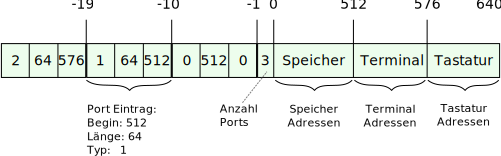
\includegraphics{img/Bus-Adressverteilung}
 \caption[Adressraumverteilung im Bussystem]
         {Adressraumverteilung im Bussystem}
 \label{fig:Bus-Adressraumverteilung}
\end{figure} 



\subsubsection{Positive Adressen}

Der Speicher bekommt einen Adressraum, der bei der Adresse Null anfängt. Die
Größe seines Adressraums ist von den Adressraum-Bedarf der anderen Ports und
von der eigenen Speicherkapazität (Adressraum-Bedarf) begrenzt. 
Nach dem Adressraum des Speichers befinden sich die Adressräume der anderen
Ports, normalerweise in der Reihenfolge ihrer Typkennung, die im Abschnitt 
\ref{subsec:Bus-Ports} auf Seite \pageref{subsec:Bus-Ports} angegeben sind.

Reicht der gesamte Adressraum  nicht für alle Ports, so wird der Adressraum
des Speichers gekürzt, bis der Bedarf aller Ports mit einem festen
Adressraum-Bedarf erfüllt ist.


